\documentclass[border=5mm]{standalone}
\usepackage{tkz-euclide}
\usetkzobj{all}
\begin{document}
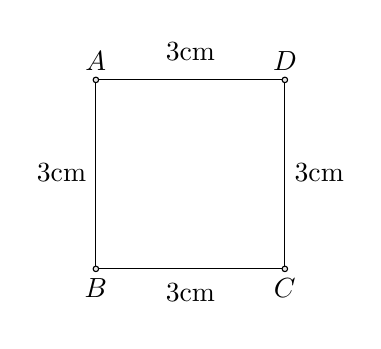
\begin{tikzpicture}[scale=.8]

\tkzDefPoint(0,0){B} \tkzDefPoint(3,0){C}
\tkzDefPoint(3,3){D} \tkzDefPoint(0,3){A}

\draw (0,0) rectangle (3,3);
\tkzDrawPoints(A,B,C,D)
\tkzLabelPoints[below](C,B)
\tkzLabelPoints[above](A,D)
%\tkzMarkRightAngle[fill=blue!20,size=0.5](A,B,C)

\node [left] at (0,1.5) {\strut 3cm};
\node [below] at (1.5,0) {\strut 3cm};
\node [right] at (3,1.5) {\strut 3cm};
\node [above] at (1.5,3) {\strut 3cm};


\end{tikzpicture}
\end{document}
\grid
\grid
\grid
